\section*{Схема экспериментальной установки}

\begin{wrapfigure}{l}{0.29\textwidth}
	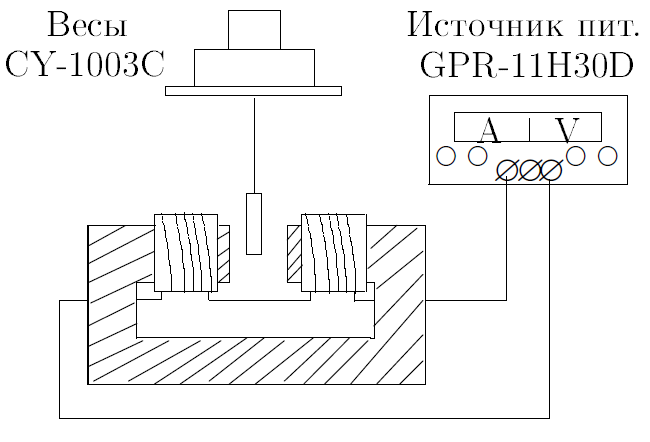
\includegraphics[width=\linewidth]{../res/scheme.png}
	\caption{Схема экспериментальной установки.}
	\label{img:scheme}
\end{wrapfigure}

Схема экспериментальной установки представлена на рис.~\ref{img:scheme}. Исследуемый образец подвешивают за тонкую нерастяжимую нить к чувствительному элементу аналитических весов. Показания весов обнуляют, и поэтому при дальнейших измерениях они будут показывать значение магнитной силы действующей на образец. Величину магнитного поля можно регулировать, изменяя ток через электромагнит, с помощью источника питания.